\documentclass{article}
\usepackage[utf8]{inputenc}

% Packages
\usepackage{amsmath,amssymb}
\usepackage{bm}% boldmath
\usepackage{listings} % Code block (source code) \begin{lstlisting} 
\usepackage{natbib}
\usepackage{graphicx}
\usepackage{lmodern}
\usepackage[usenames,dvipsnames,svgnames,table]{xcolor}
\usepackage[textwidth=16cm,textheight=23cm]{geometry}
\usepackage{subfig} % Subfigures. Uses \subfloat[captions text]{figure}
\usepackage{hyperref} % Enables \url{url} and \href{url}{name}
\usepackage{multicol} % \begin{columns}

% Commands
\newcommand{\code}[1]{\texttt{#1}} % \code{inline code}
\newcommand{\expval}[1]{\langle #1 \rangle} %
\renewcommand{\theequation}{\arabic{section}.\arabic{equation}} % Book format equation
\renewcommand{\thefigure}{\arabic{section}.\arabic{figure}} % Book format figure
\renewcommand{\vec}[1]{{\bf #1}} % Lars likes this better than arrow

% Set page attribution
\setlength{\parindent}{0pt}


% PSTRICKS
\usepackage{pstricks,pst-node,pst-tree} % includes graph additions
\usepackage{pst-pdf}	% Compiles the pictures
\usepackage{pst-node}
\usepackage{pst-plot}
\usepackage{pst-3dplot}
%\usepackage{pstricks-add,babel}


% ***************************************************
% HEADER INFORMATION

\title{Pylab (Matplotlib) Introduction}
\author{Molecular Statistics}
\date{2014}

% ***************************************************

\begin{document}

%commentstyle=\color{gray},              % Comments font
%basicstyle=\small,                      % Code font, Examples: \footnotesize, \ttfamily


\lstset{
language=Python,                        % Code langugage
commentstyle=\color{gray},              % Comments font
basicstyle=\small\ttfamily,             % Code font, Examples: \footnotesize, \ttfamily
keywordstyle=\bfseries\color{blue},
stringstyle=\color{orange},
numbers=left,                           % Line nums position
numberstyle=\tiny,                      % Line-numbers fonts
stepnumber=1,                           % Step between two line-numbers
numbersep=5pt,                          % How far are line-numbers from code
frame=none,                             % A frame around the code
tabsize=4,                              % Default tab size
captionpos=b,                           % Caption-position = bottom
breaklines=true,                        % Automatic line breaking?
breakatwhitespace=false,                % Automatic breaks only at whitespace?
showspaces=false,                       % Dont make spaces visible
showtabs=false,                         % Dont make tabls visible
belowskip=10pt,
showstringspaces=false
}

%basicstyle=\footnotesize\ttfamily,
%keywordstyle=\bfseries\color{green!40!black},
%commentstyle=\itshape\color{purple!40!black},
%identifierstyle=\color{blue},
%stringstyle=\color{orange},



% ***************************************************
% BEGIN DOCUMENT
% ***************************************************

\maketitle

\section{Introduction}

Pylab is a module for Python used for plotting, which utilizes
another module called Matplotlib. It is very useful for plotting all kinds
of data and is extremely customizable.  See the gallery
\href{http://matplotlib.org/gallery.html}{matplotlib.org/gallery.html}, or
\href{http://webloria.loria.fr/~rougier/teaching/matplotlib/}{webloria.loria.fr/\~{}rougier/teaching/matplotlib}
for examples. \\

In this short introduction we will go through small useful examples with
provided code. For more advanced examples (like 3D plots), see the links above
or do a Google-search. \\

All the examples below will be using the python package \code{pylab}, and
must thus be included in your script. This is done by including

\begin{lstlisting}
import pylab
\end{lstlisting}

in the head of the \code{.py}-file.\\

To illustrate the result of a plot/graph, you can either show it in a new window or save the
plot as an image.

\begin{lstlisting}
# Show the result in a new window
pylab.show()

# Save the result in a file
pylab.savefig('this_figure.png')
\end{lstlisting}

% Full list:
% emf, eps, jpeg, jpg, pdf, png, ps, raw, rgba, svg, svgz, tif, tiff

The \code{savefig()} method can save to
\code{.png},
\code{.eps},
\code{.svg},
as well as
\code{.pdf}.\\

When creating multiple plots in the same script, remember to {\em clear figure} after each plot,
using

\begin{lstlisting}
pylab.clf()
\end{lstlisting}

which will erase all previous work done in pylab.



\newpage
\section{Examples}

\subsection{XY}

A simple example is to plot $x$ and $y$ coordinates
based on two simple python lists.

\begin{multicols}{2}

\begin{lstlisting}
import pylab

x = range(1, 20)
y = [i**2 for i in x]

# Plot x- and y coordinates
pylab.plot(x, y)
pylab.savefig('xy_figure.png')

\end{lstlisting}
\columnbreak
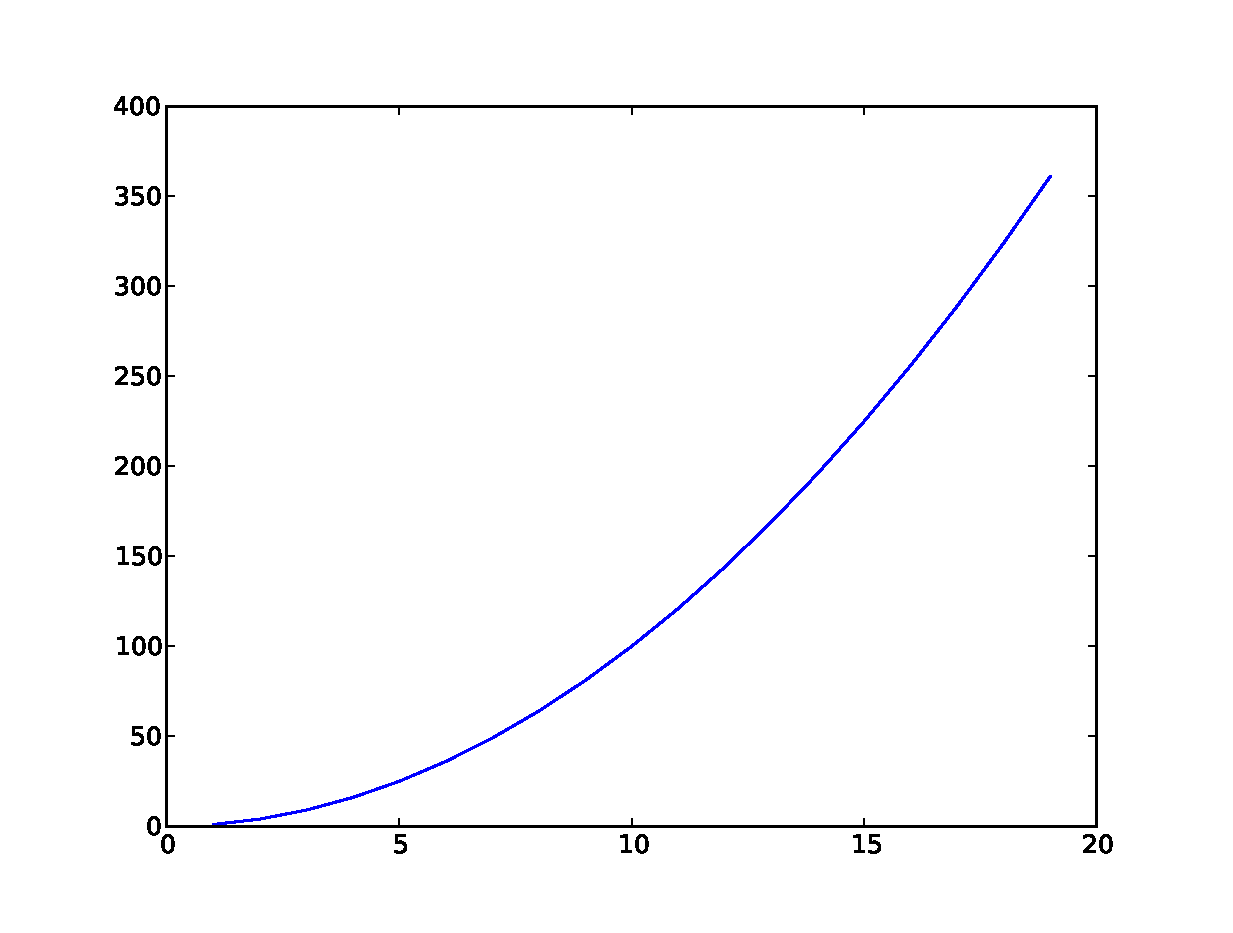
\includegraphics[width=0.6\textwidth]{py/xy_figure.eps}
\end{multicols}


\newpage
\subsection{Titles and labels}

However a graph is worth nothing without title and axis-labels,
which can be included by the following syntax.
It is also possible to include latex code in the strings.

\begin{multicols}{2}

\begin{lstlisting}
import pylab

x = range(1, 20)
y = [i**2 for i in x]

# Plot x- and y coordinates
pylab.plot(x, y)

# Set title
pylab.title("Wow, Nice graph")

# Axis
pylab.xlabel('kcal/mol')
pylab.ylabel('$\hat \lambda R^2$')

pylab.savefig('figure_name.png')
\end{lstlisting}
\columnbreak
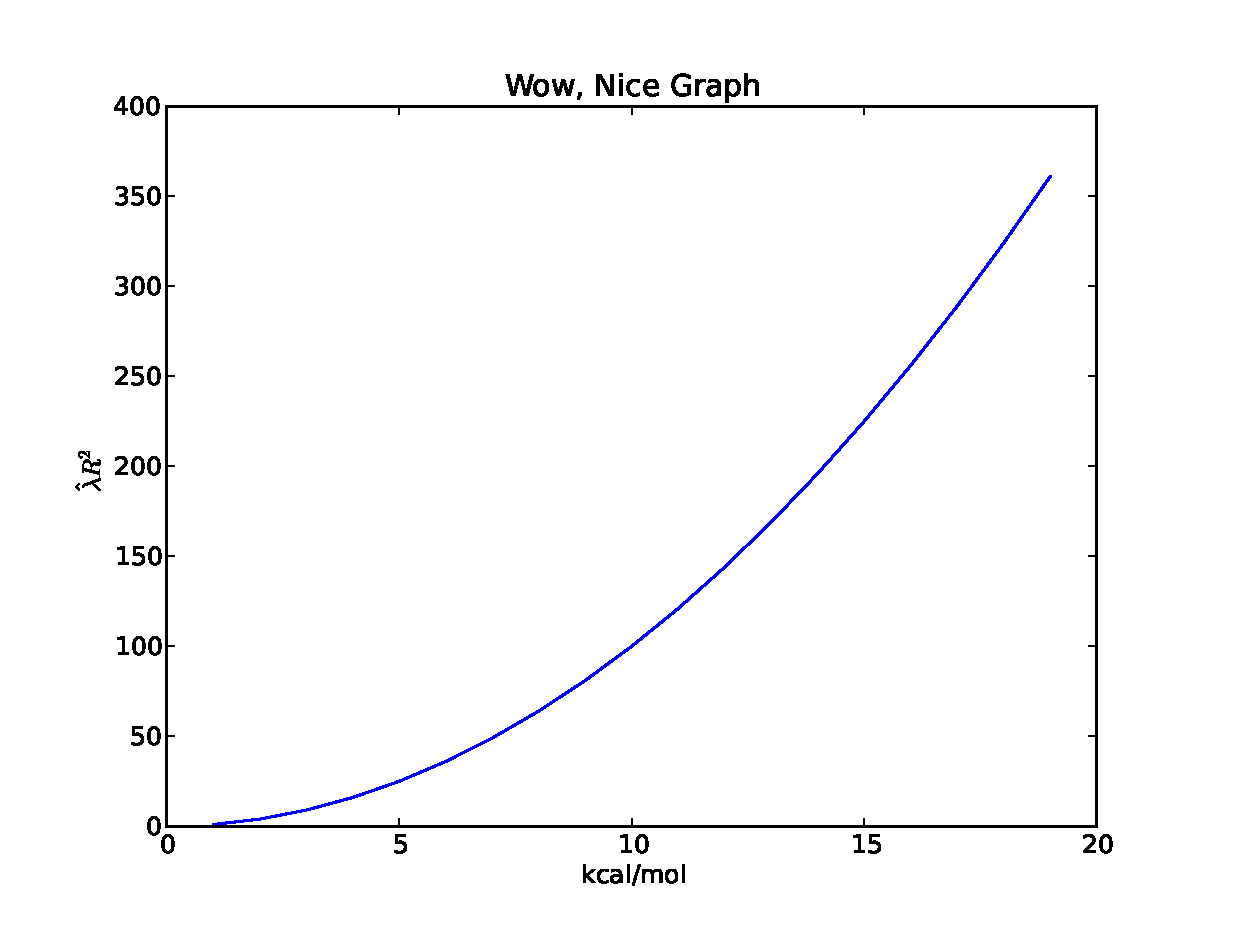
\includegraphics[width=0.6\textwidth]{py/figure_title.eps}
\end{multicols}

\subsection*{}

Text can also be inserted into the figure, for example

\begin{multicols}{2}

\begin{lstlisting}
import pylab

x = range(1, 20)
y = [i**2 for i in x]

# Plot x- and y coordinates
pylab.plot(x, y)

# Set title
pylab.title("Wow, Nice graph")

# Axis
pylab.xlabel('kcal/mol')
pylab.ylabel('$\hat \lambda R^2$')

# Text
pylab.text(5, 200, r'$\mu=100,\ \sigma=15$')

pylab.savefig('figure_name.png')
\end{lstlisting}
\columnbreak
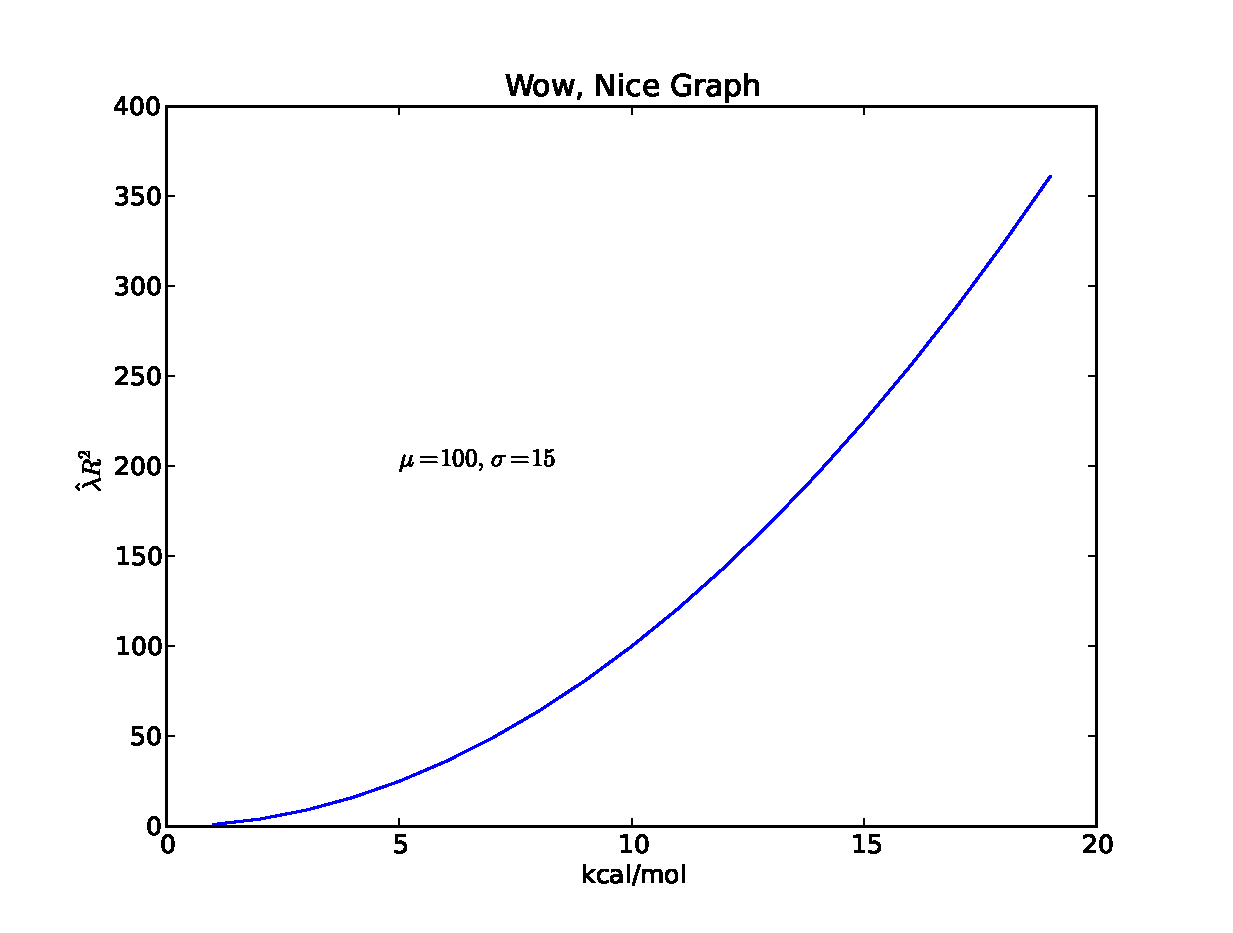
\includegraphics[width=0.6\textwidth]{py/figure_title_text.eps}
\end{multicols}



\newpage
\subsection{Multiple lines}

Plotting multiple datasets in the same figure
can be done by choosing a color and
a line style for the plot.
See appendix A for a full list of
colors and line styles.

\begin{multicols}{2}

\begin{lstlisting}
import pylab
import math

x = numpy.arange(0, 14, 0.1)
y_cos = [math.cos(i) for i in x]
y_sin = [math.sin(i) for i in x]

# Insert x and y coordinates
# with a red and blue line
pylab.plot(x, y_cos, 'r-')
pylab.plot(x, y_sin, 'b-')

pylab.savefig('figure_sincos1.png')

\end{lstlisting}
\columnbreak
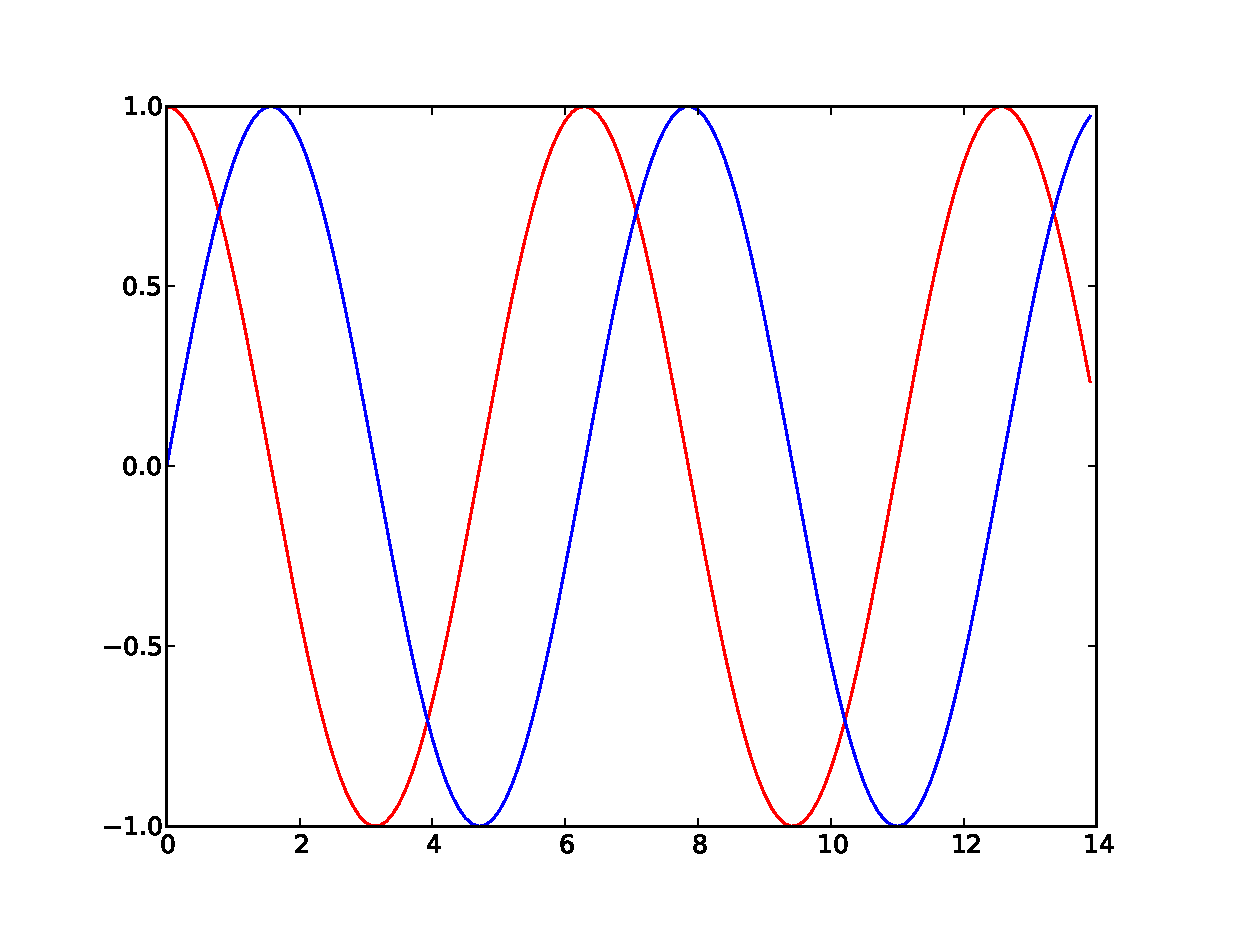
\includegraphics[width=0.6\textwidth]{py/figure_sincos1.eps}
\end{multicols}

Having labels/legends on the plots can be fairly important. This
is done by assigning each plot a label, and inserting them in the figure by using the legend
command.
Note that the location of the legend box can be set by changing the string location.


\begin{multicols}{2}

\begin{lstlisting}
import pylab
import math

x = numpy.arange(0, 14, 0.1)
y_cos = [math.cos(i) for i in x]
y_sin = [math.sin(i) for i in x]

pylab.plot(x, y_cos, 'r-', label="Cos function")
pylab.plot(x, y_sin, 'b-', label="Sin function")

pylab.legend(loc='upper left')

pylab.savefig('figure_sincos2.png')

\end{lstlisting}
\columnbreak
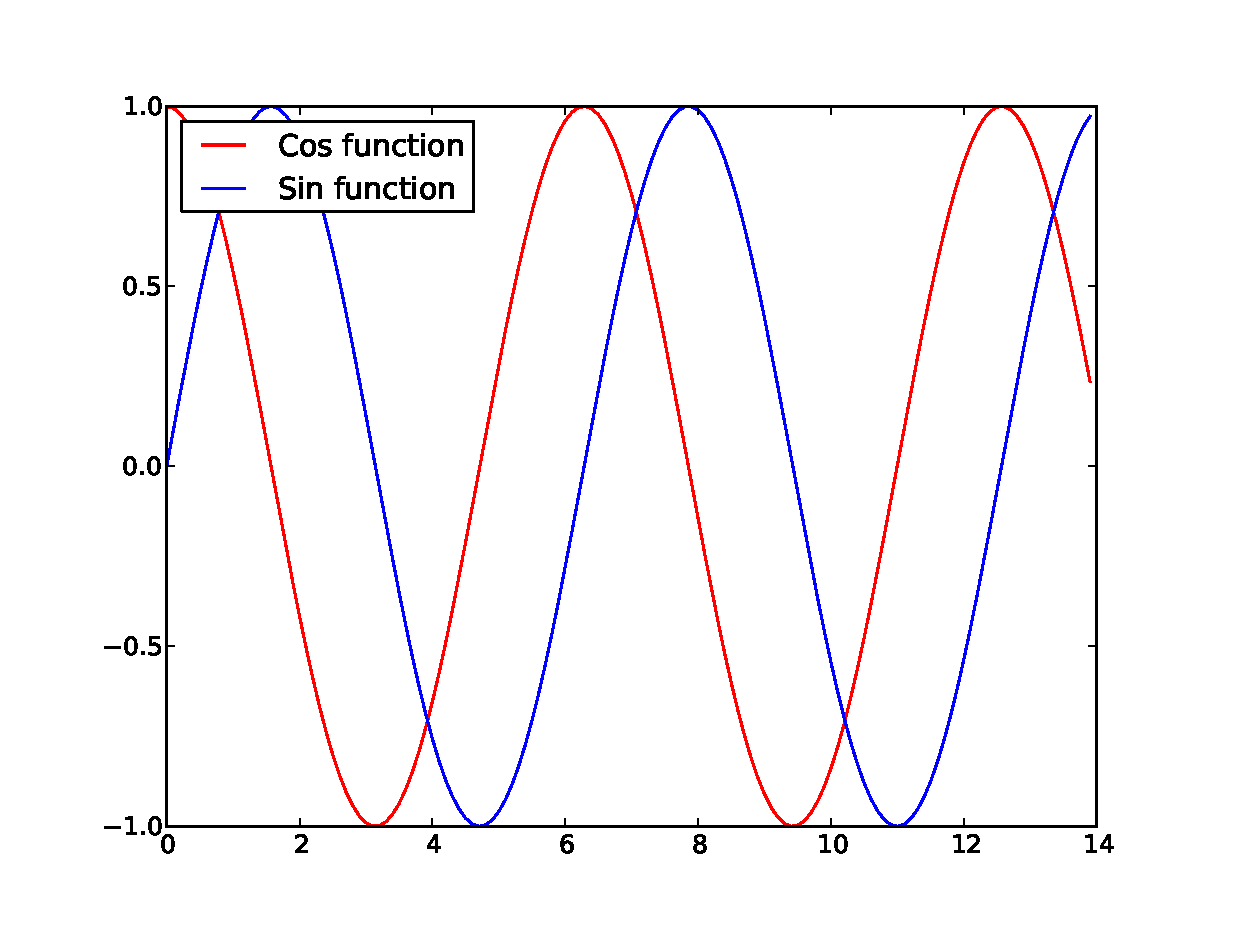
\includegraphics[width=0.6\textwidth]{py/figure_sincos2.eps}
\end{multicols}






%%%%%%%%%%%%%%%%%


% TODO EXAMPLES
% xlim(X.min()*1.1, X.max()*1.1)
%ylim(C.min()*1.1, C.max()*1.1)


% import matplotlib matplotlib.use("Agg")



\appendix
\newpage

\section{Plot styling}

\begin{multicols}{2}

\subsection{Colors}

\begin{tabular}{ l l }
b & blue \\
g & green \\
r & red \\
c & cyan \\
m & magenta \\
y & yellow \\
k & black \\
w & white
\end{tabular}

\columnbreak

\subsection{Line styles}

\begin{tabular}{ l l }
0 & tickleft\\
1 & tickright\\
2 & tickup\\
3 & tickdown\\
4 & caretleft\\
D & diamond\\
6 & caretup\\
7 & caretdown\\
s & square\\
| & vline\\
x & x\\
5 & caretright\\
\_ & hline\\
\^{} & triangle up\\
d & thin diamond\\
h & hexagon1\\
+ & plus\\
* & star\\
, & pixel\\
o & circle\\
. & point\\
'1' & tri down\\
p & pentagon\\
'3' & tri left\\
'2' & tri up\\
'4' & tri right\\
H & hexagon2\\
v & triangle down\\
'8' & octagon\\
\textless & triangle left\\
\textgreater & triangle right
\end{tabular}

\end{multicols}



% ***************************************************
% END DOCUMENT
% ***************************************************

\end{document}

